\documentclass[article,12pt,openright,oneside,a4paper,brazil]{abntex2}
\usepackage[utf8]{inputenc}
\usepackage[brazil]{babel}
\usepackage{tgpagella}
\usepackage{indentfirst}
\usepackage[alf, bibjustif]{abntex2cite}
\usepackage{graphicx}
\usepackage{float}
\usepackage{pdfpages}
\hypersetup{pdfborder=0 0 0}

\setlength{\parindent}{1.25cm}
\setlength{\parskip}{0cm}

\begin{document}

\setcounter{page}{1}
\pagenumbering{arabic}

\section*{\textbf{Assignment 0}: Esboços de Visualizações}
\subsection*{Visualização de Dados \\ Felipe Marques Esteves Lamarca \\}

    \begin{description}
        \item[Pergunta:] Existe algum padrão de variação na criminalidade ao longo dos meses do ano? \\

        \item[Esboço 1:] Gráfico de linha representando o número absoluto de crimes por mês, somando todas as cidades do \textit{dataset}.        
    \end{description}

    \begin{figure}[H]
        \centering
        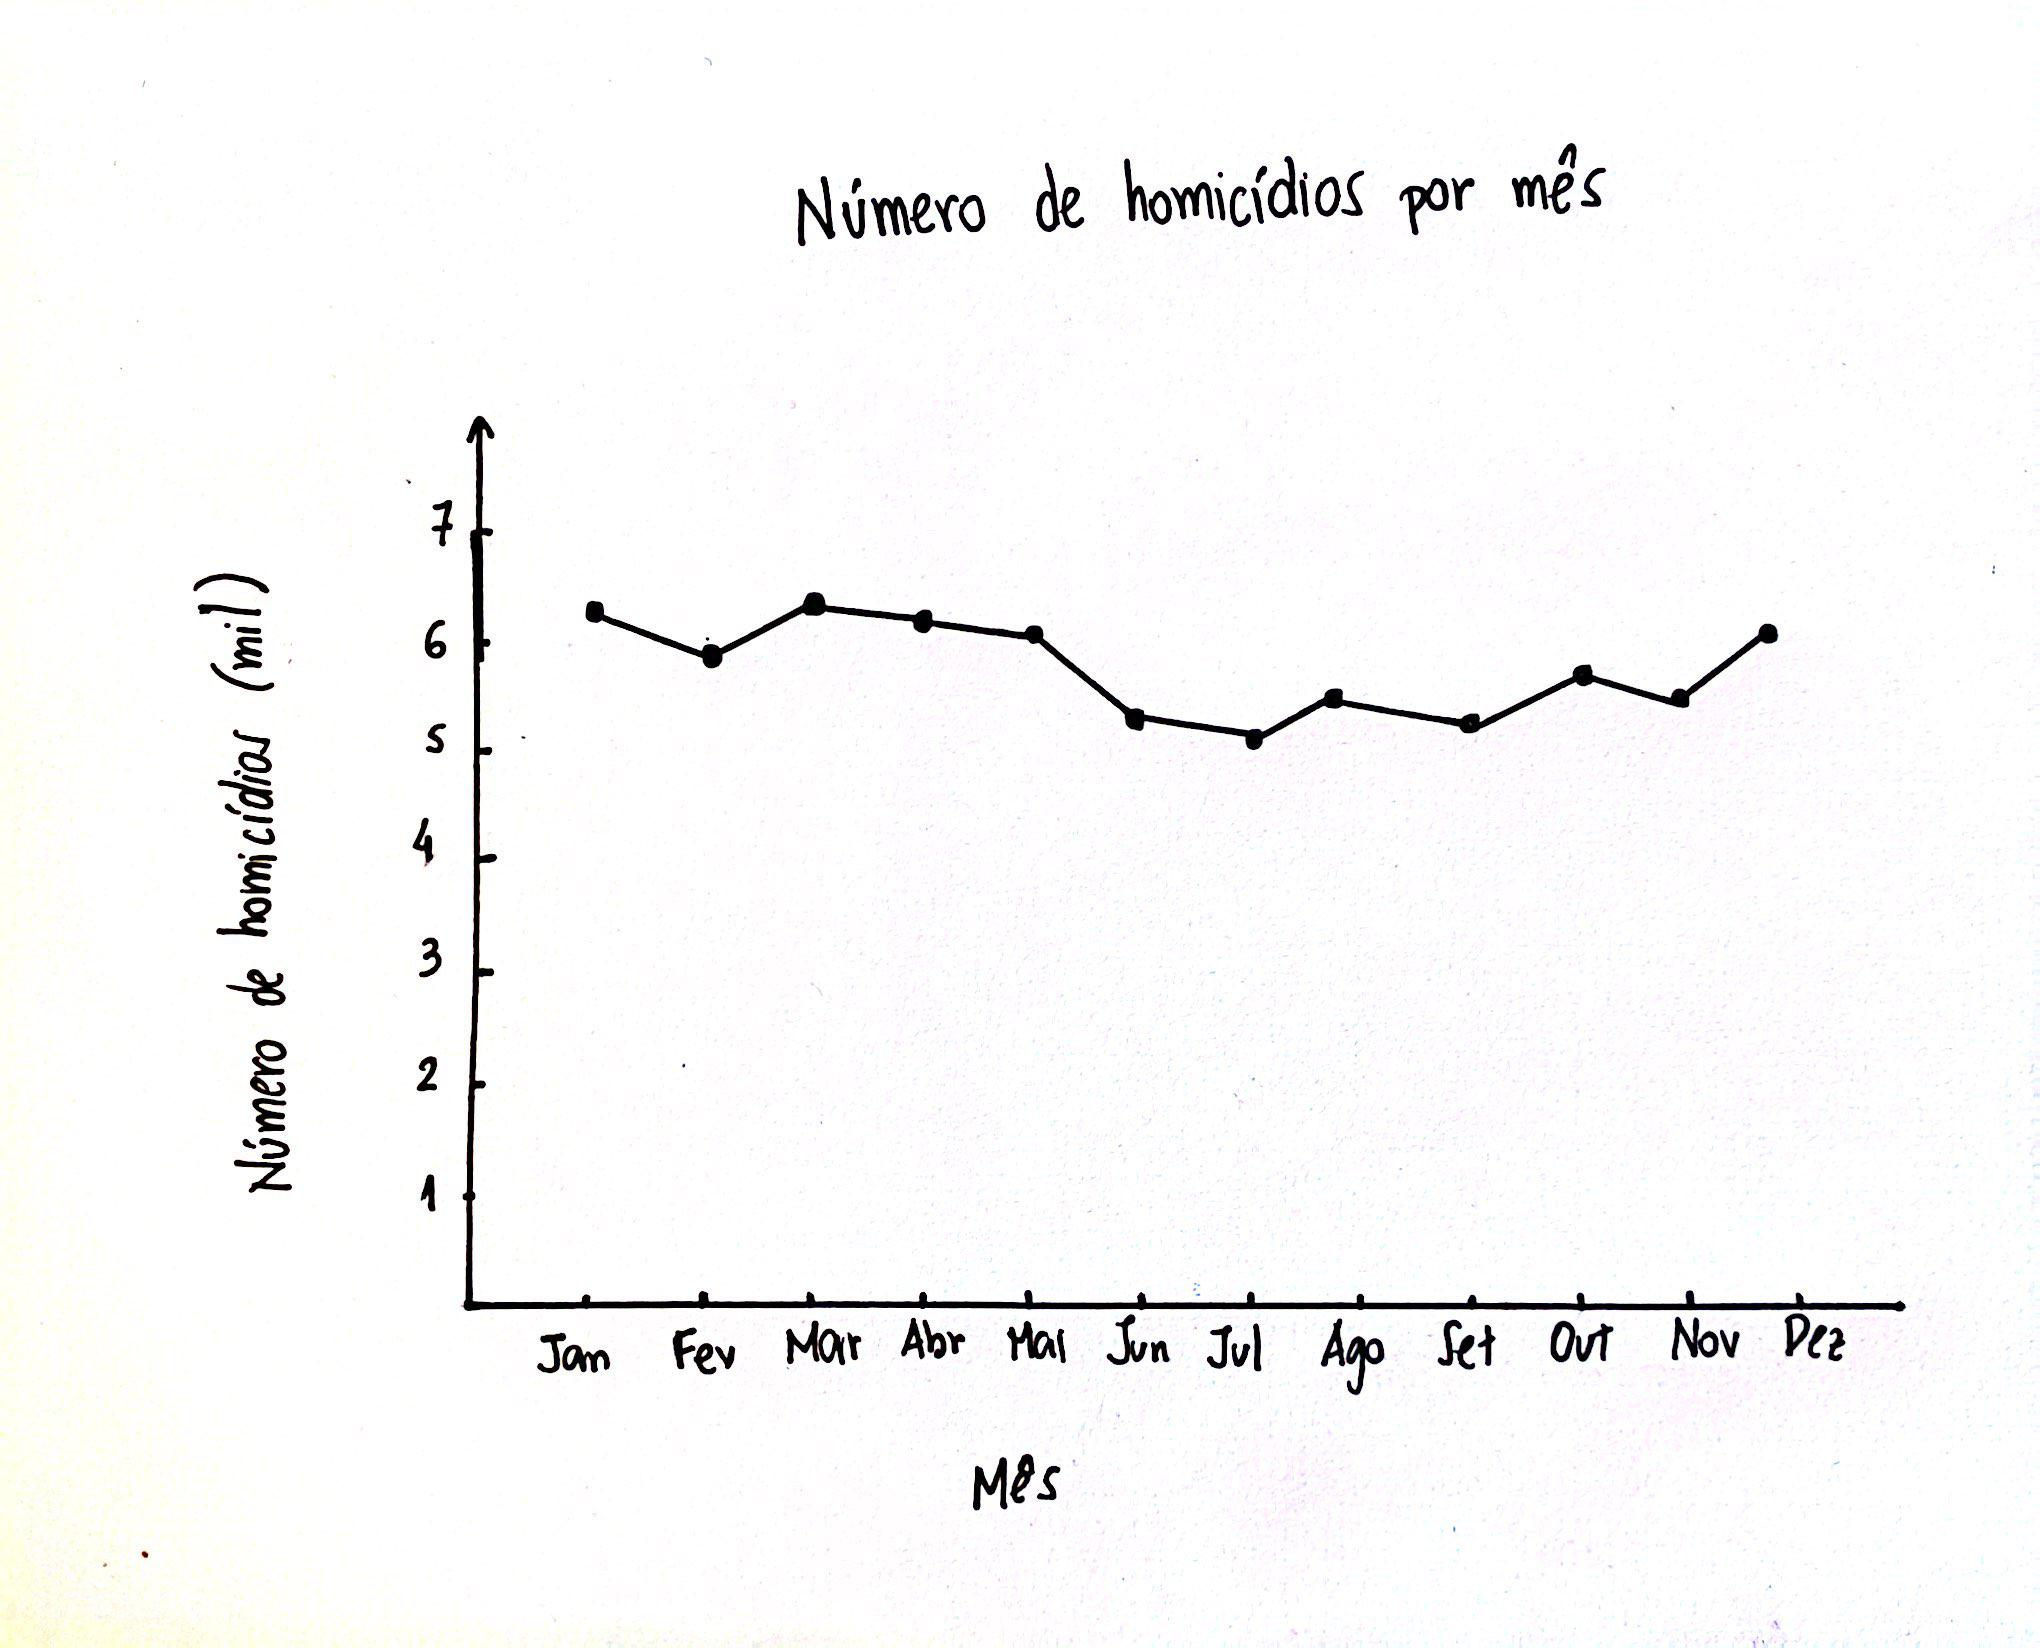
\includegraphics[width=15cm]{graphs/graph1.jpg}
        \caption{Esboço 1}
        \label{fig:esboco_1}
    \end{figure}

    O objetivo dessa visualização, em particular, é observar como se comporta a distribuição de crimes ao longo dos meses. Em outras palavras, é um esboço que permite avaliar se existem meses ``menos perigosos'' que outros do ponto de vista de número total de homicídios. É possível, em uma dimensão mais geral, observar que há uma queda na ordem de algumas centenas de casos por volta dos meses entre junho e setembro, com posterior crescimento no final e no início dos anos. Uma limitação desse gráfico é que a representação geral, sem considerar cidade por cidade, não possibilita uma análise mais específica. 

    \begin{description}
        \item[Esboço 2:] Gráfico de barras com o percentual de variação do número de casos de um mês em relação ao anterior.
    \end{description}

    \begin{figure}[H]
        \centering
        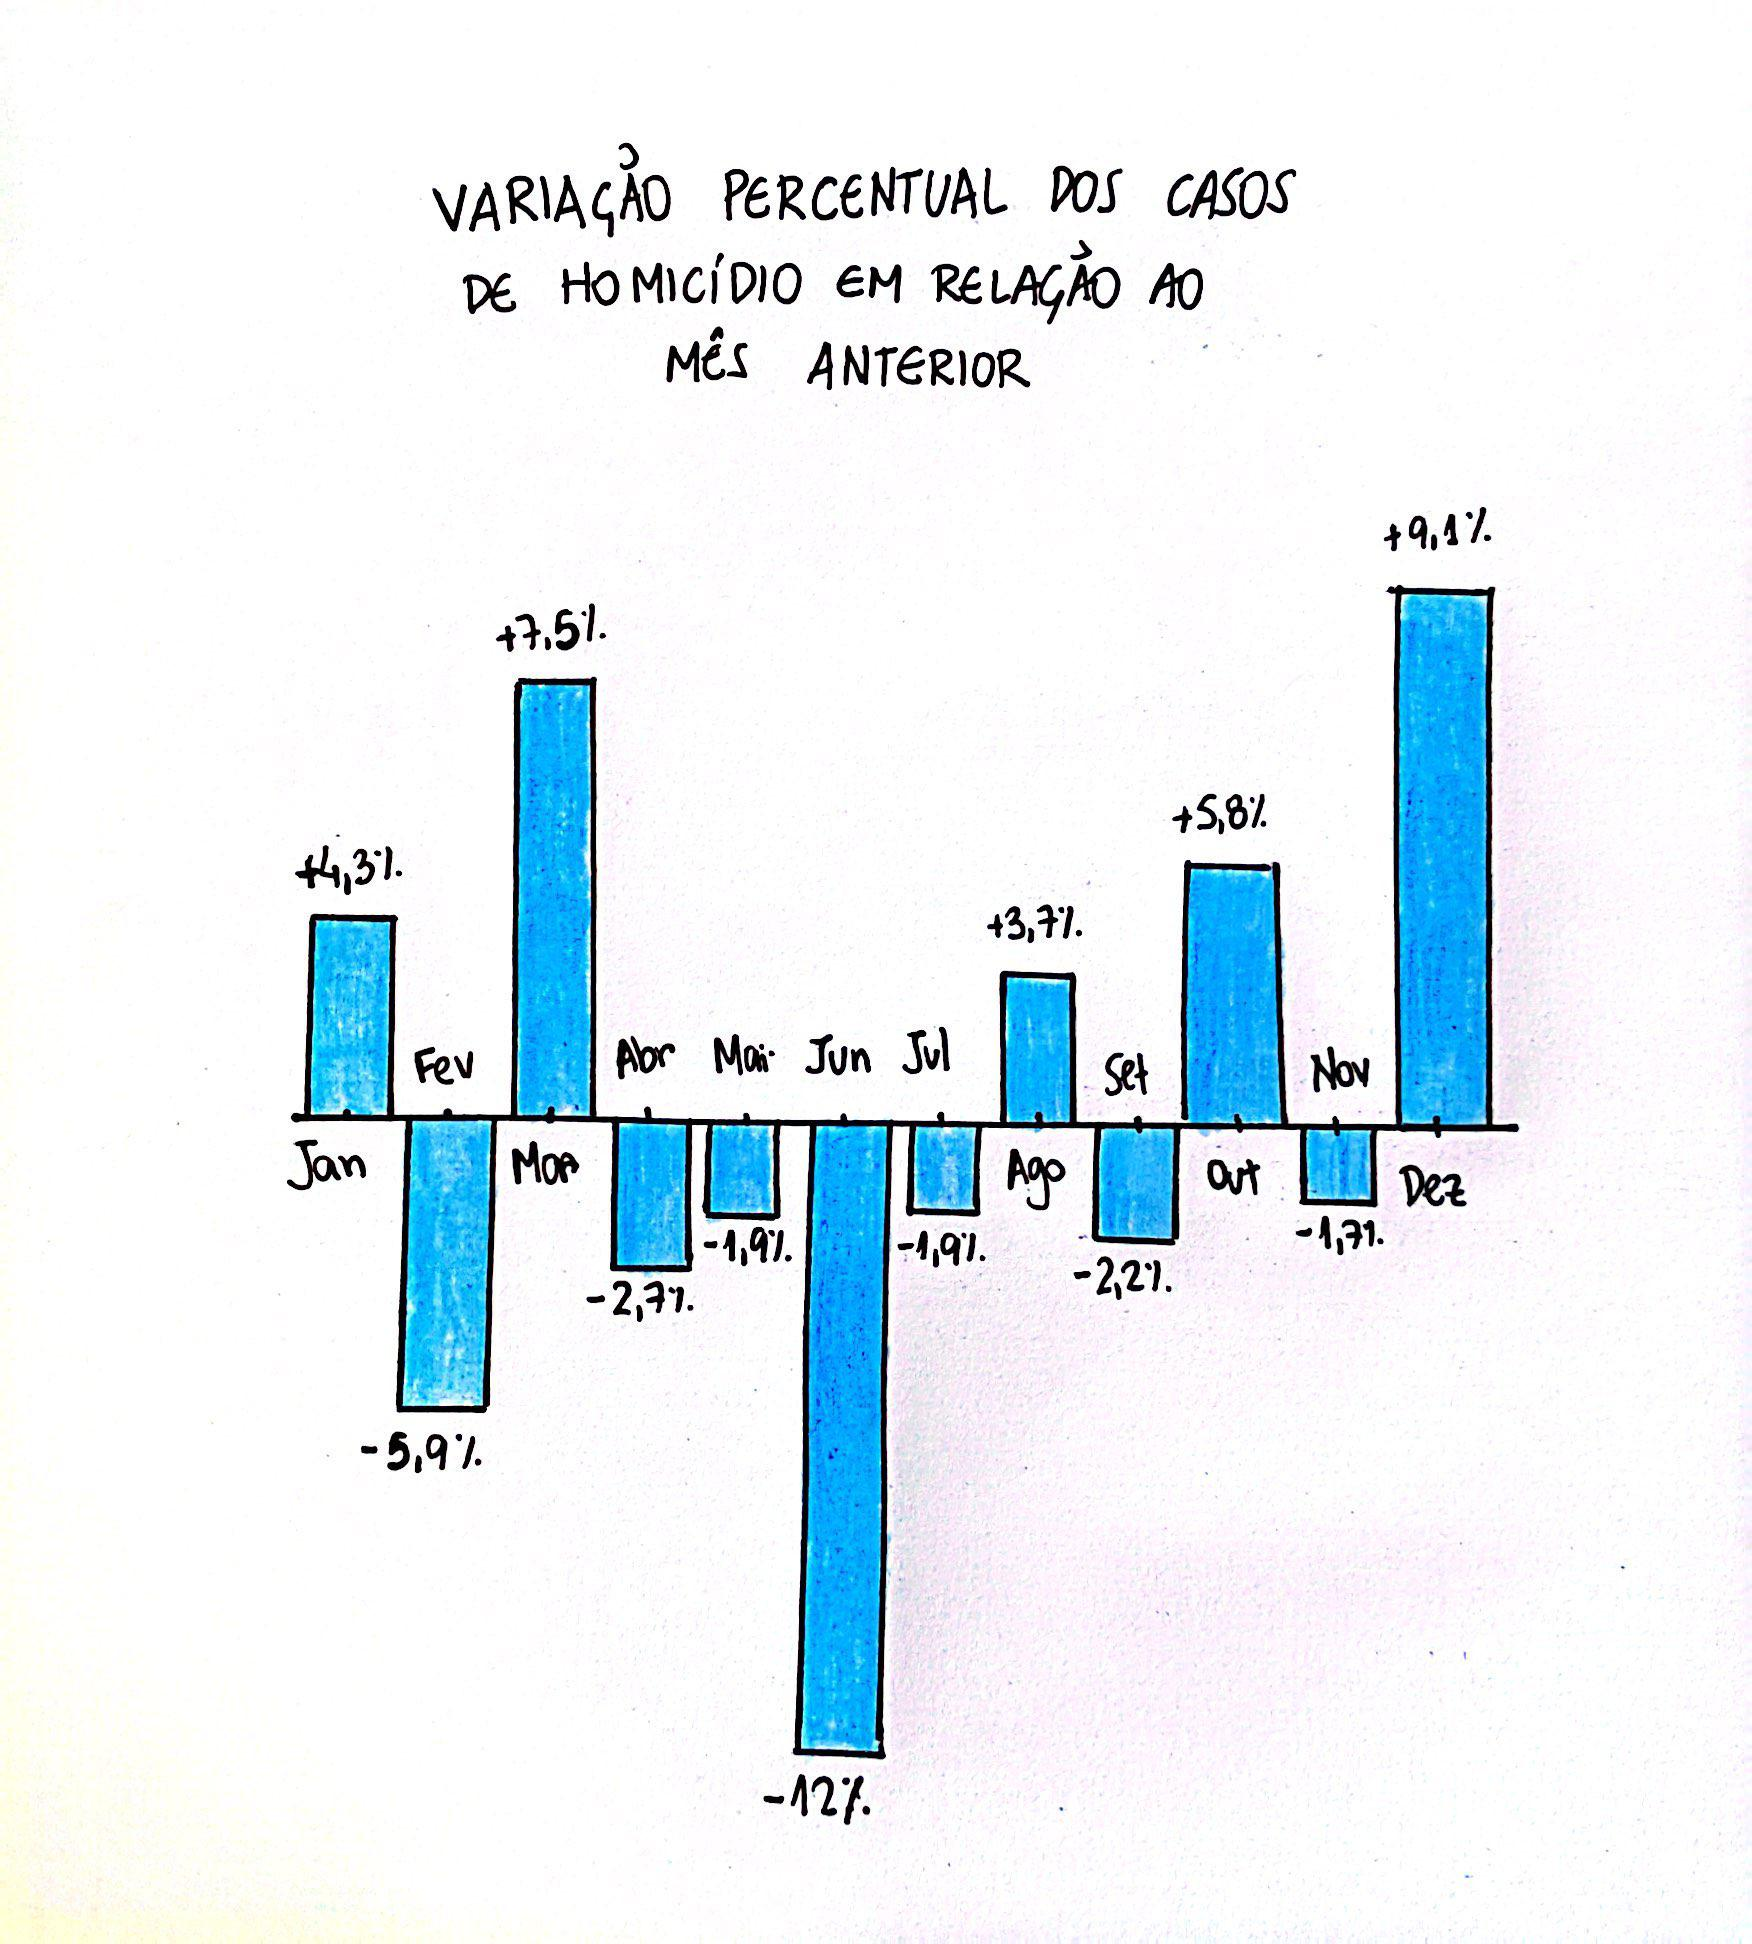
\includegraphics[width=15cm]{graphs/graph2.jpg}
        \caption{Esboço 2}
        \label{fig:esboco_2}
    \end{figure}

    O segundo esboço complementa o primeiro na medida em que quantifica as variações no número de um homicídio em determinado mês, levando em consideração o valor observado no mês anterior. O objetivo, nesse caso, é verificar quando há as maiores quedas ou crescimentos percentuais, o que pode ser um indicativo de mudança na dinâmica da criminalidade ao longo do ano. Naturalmente, como esperado, a queda mais acentuada ocorre na virada de maio para junho, e volta a crescer mais constantemente a partir de outubro. É claro, trata-se de uma análise limitada, já que a representação é percentual e não em valores absolutos. Ainda assim, é uma boa forma de observar tendências de mudança ao longo do ano. Novamente, a representação desconsidera a análise por cidades, e, como a Capital possui os maiores números de casos, é possível questionar se o gráfico segue uma tendência mais particular do que geral. O esboço 3 tenta sanar essa questão.

    \begin{description}
        \item[Esboço 3:] Gráfico de barras com o percentual de variação do número de casos de um mês em relação ao anterior, por cidade\footnote{Por questões de tamanho, este esboço foi adicionado ao final do documento}.
    \end{description}

    O objetivo nesse caso é avaliar se o padrão de variação na criminalidade se repete em cada uma das cidades, ou se há diferenças entre elas. Como comentado, a análise agregada dificulta análises particulares na medida em que o número de casos na Capital é muito mais alto em todos os meses. Portanto, o esboço elaborado segue o padrão de um esquema de grades, em que cada bloco corresponde à uma cidade do \textit{dataset} e realiza o mesmo \textit{plot} do gráfico anterior para cada uma delas. Com isso, é possível comunicar uma série de informações mais específicas e confirmar outras mais gerais. Por exemplo, a queda de casos de homicídio em meados de cada ano realmente é um padrão comum a todas elas, mas nem todas iniciam o ano com aumento de casos, como Campinas e Sorocaba.

    \begin{description}
        \item[Discussão geral:] Os 3 esboços apresentados ao longo desta tarefa foram pensados de forma que a análise de cada um deles fosse complementar, dando uma visão geral da variação da criminalidade ao longo dos meses. Se o gráfico inicial, com números absolutos, fornece um quadro geral do número de casos, ele desconsidera as características mais particulares de cada cidade. Ao mesmo tempo, ele não dá o enfoque necessário à variação entre os meses, informação fundamental para encontrar pontos de inflexão na dinâmica de homicídios nos territórios e, na prática, para responder à questão enunciada no início deste documento. É isso que os esboços posteriores apresentam, complementando a primeira informação e tornando a análise mais completa. Possíveis direcionamentos de exploração dos dados poderiam envolver, por exemplo, uma análise que também considere a dimensão territorial em primeiro plano, focando nas diferenças entre as cidades no que diz respeito ao índice de homicídios. Essa questão foi menos explorada em detrimento da dimensão temporal.
    \end{description}

    \newpage
    
    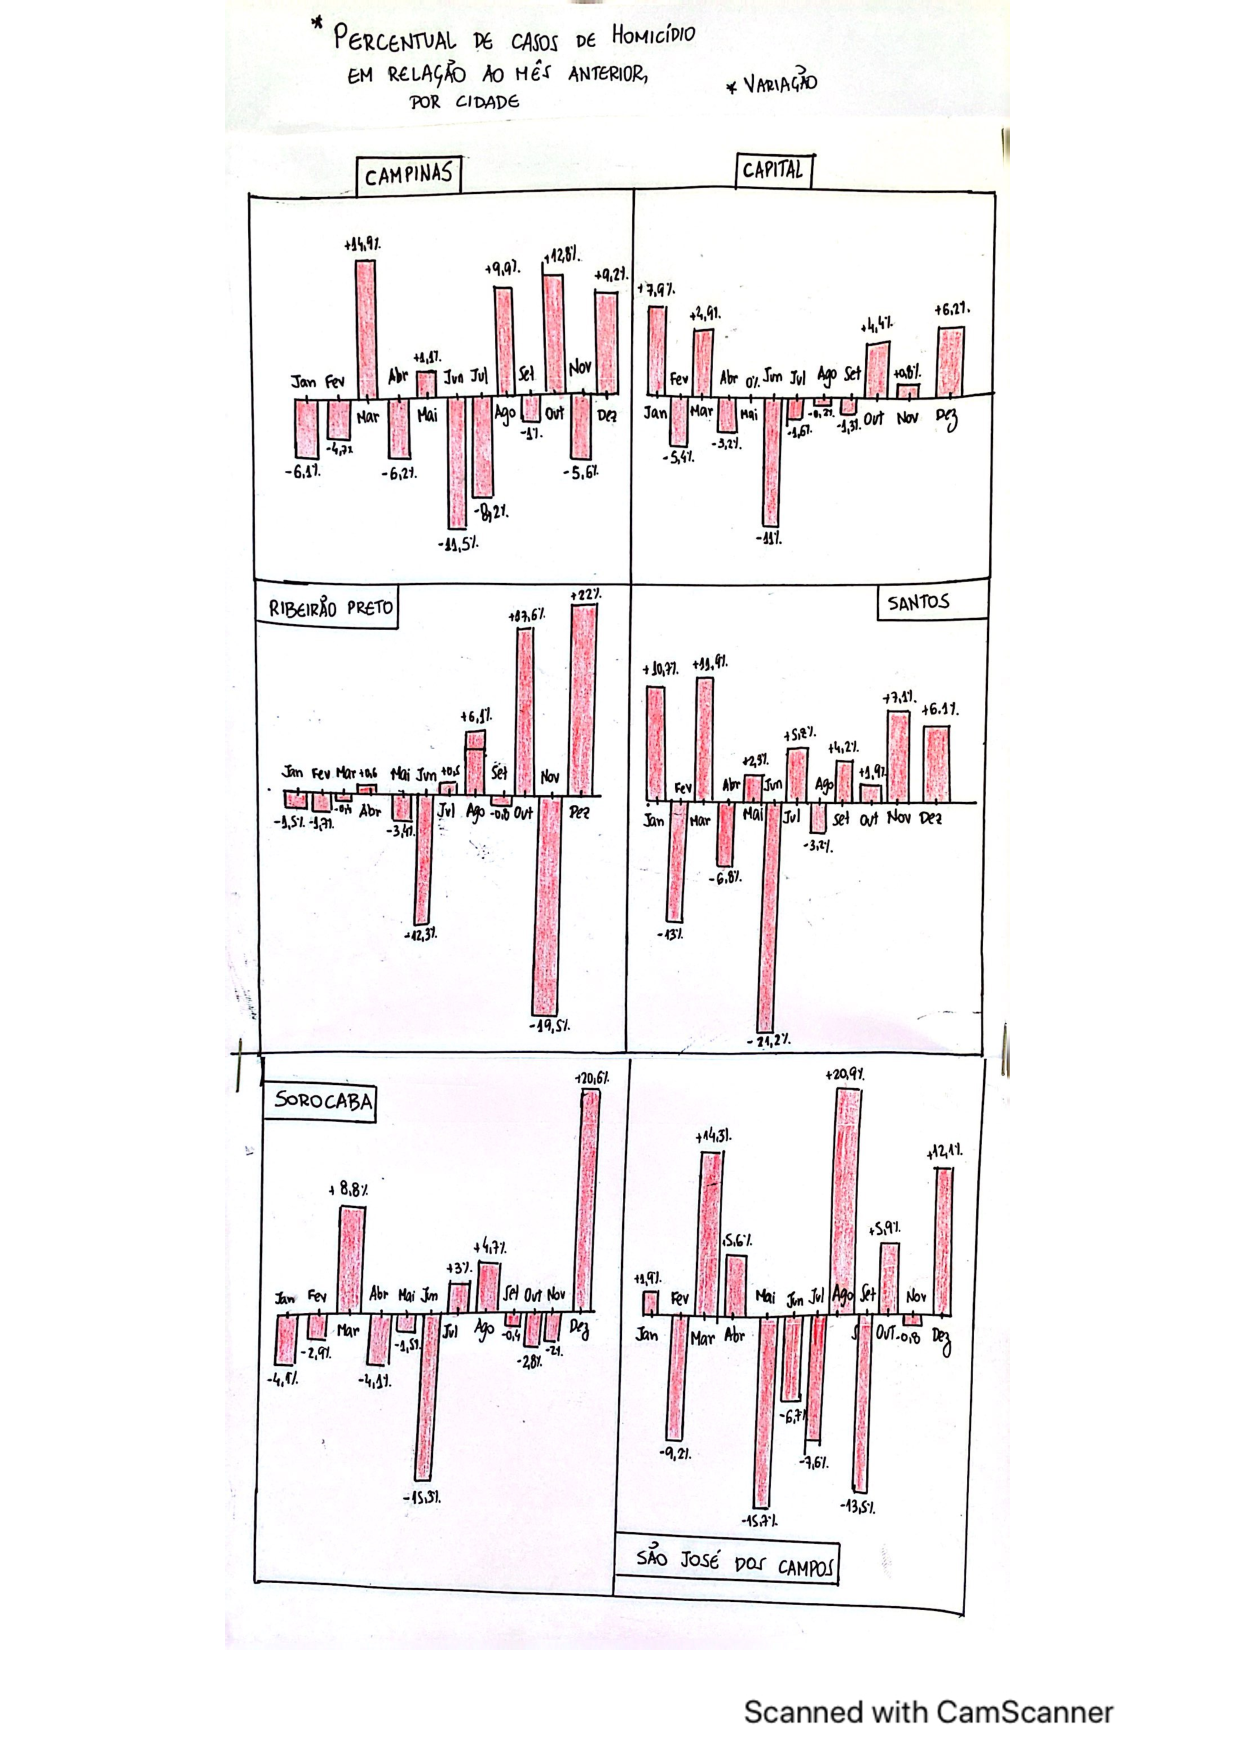
\includepdf{graphs/graph3.pdf}

    

\end{document}
